\documentclass[border=10pt,tikz]{standalone}
\usepackage{tikz}
\usepackage{xcolor}
\usepackage[T1]{fontenc}
\usepackage{lmodern}
\usetikzlibrary{positioning,arrows.meta,decorations.pathreplacing,calc,fadings,patterns,shadows}

\definecolor{ink}{HTML}{0E1116}
\definecolor{inksoft}{HTML}{3A3F47}
\definecolor{inkmute}{HTML}{6A7079}
\definecolor{textc}{HTML}{2563EB}
\definecolor{audioc}{HTML}{EA580C}
\definecolor{accentc}{HTML}{7C3AED}
\definecolor{audiogreen}{HTML}{059669}
\definecolor{linec}{HTML}{CFC9B8}
\definecolor{soft}{HTML}{F3F1EA}
\definecolor{warn}{HTML}{B91C1C}

\begin{document}
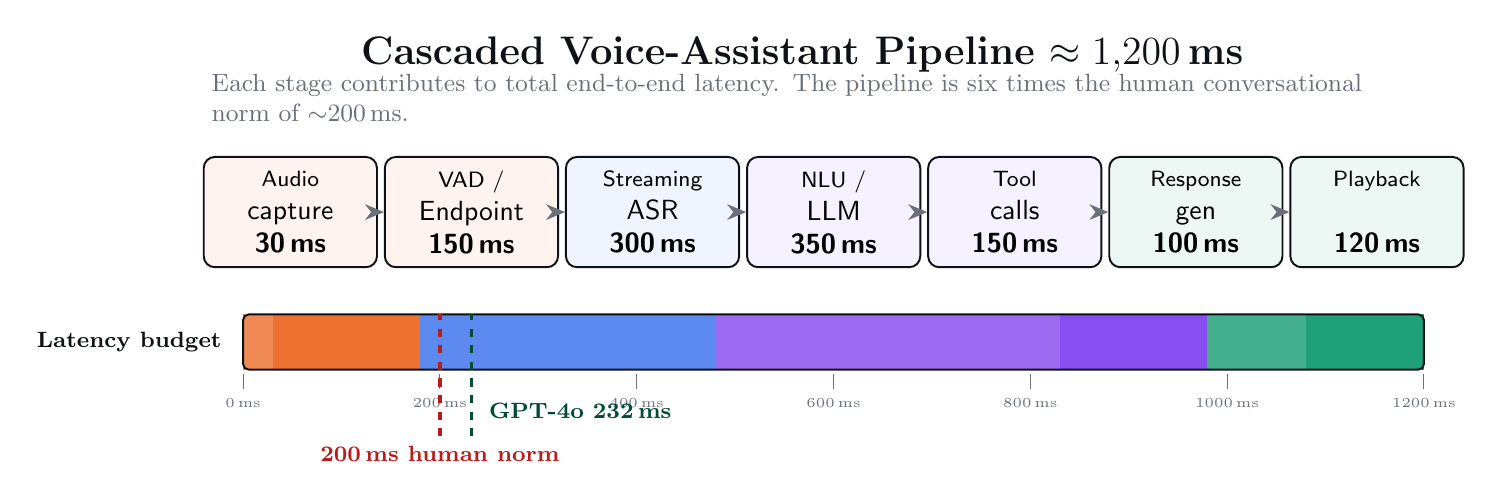
\begin{tikzpicture}[
  font=\sffamily,
  every node/.style={font=\sffamily},
  stage/.style={
    rectangle, rounded corners=4pt,
    draw=ink, line width=0.7pt,
    fill=white,
    minimum height=14mm, minimum width=22mm, align=center,
    inner sep=4pt
  }
]

% Title
\node[font=\Large\bfseries, color=ink] at (7.5,5.6) {Cascaded Voice-Assistant Pipeline \(\approx 1{,}200\)\,ms};
\node[font=\small, color=inkmute, text width=15cm, align=left] at (7.5,5.05) {Each stage contributes to total end-to-end latency. The pipeline is six times the human conversational norm of \(\sim\)200\,ms.};

% Stages
\node[stage, fill=audioc!7] (s1) at (1.0,3.6) {\footnotesize Audio\\capture\\\textbf{30\,ms}};
\node[stage, fill=audioc!7] (s2) at (3.3,3.6) {\footnotesize VAD /\\Endpoint\\\textbf{150\,ms}};
\node[stage, fill=textc!7]  (s3) at (5.6,3.6) {\footnotesize Streaming\\ASR\\\textbf{300\,ms}};
\node[stage, fill=accentc!7] (s4) at (7.9,3.6) {\footnotesize NLU /\\LLM\\\textbf{350\,ms}};
\node[stage, fill=accentc!7] (s5) at (10.2,3.6) {\footnotesize Tool\\calls\\\textbf{150\,ms}};
\node[stage, fill=audiogreen!7] (s6) at (12.5,3.6) {\footnotesize Response\\gen\\\textbf{100\,ms}};
\node[stage, fill=audiogreen!7] (s7) at (14.8,3.6) {\footnotesize Playback\\\\\textbf{120\,ms}};

% Arrows between
\foreach \a/\b in {s1/s2, s2/s3, s3/s4, s4/s5, s5/s6, s6/s7} {
  \draw[->, >={Stealth[length=2.4mm,width=2.0mm]}, draw=inkmute, line width=0.5pt] (\a.east) -- (\b.west);
}

% Latency budget bar (cumulative). Convert ms to x-coordinates.
% origin x=0.4, total width = 15.0. Scale = 15/1200 = 0.0125
\pgfmathsetmacro\Lo{0.4}
\pgfmathsetmacro\Ls{0.0125}
\pgfmathsetmacro\Lh{0.7}
\pgfmathsetmacro\Ly{1.6}
\pgfmathsetmacro\Lytop{\Ly+\Lh}

% Helper: x at ms
\pgfmathsetmacro\xA{\Lo + 30*\Ls}
\pgfmathsetmacro\xB{\Lo + 180*\Ls}
\pgfmathsetmacro\xC{\Lo + 480*\Ls}
\pgfmathsetmacro\xD{\Lo + 830*\Ls}
\pgfmathsetmacro\xE{\Lo + 980*\Ls}
\pgfmathsetmacro\xF{\Lo + 1080*\Ls}
\pgfmathsetmacro\xG{\Lo + 1200*\Ls}

% Segments
\fill[audioc!70]      (\Lo, \Ly) rectangle (\xA, \Lytop);
\fill[audioc!85]      (\xA, \Ly) rectangle (\xB, \Lytop);
\fill[textc!75]       (\xB, \Ly) rectangle (\xC, \Lytop);
\fill[accentc!75]     (\xC, \Ly) rectangle (\xD, \Lytop);
\fill[accentc!90]     (\xD, \Ly) rectangle (\xE, \Lytop);
\fill[audiogreen!75]  (\xE, \Ly) rectangle (\xF, \Lytop);
\fill[audiogreen!90]  (\xF, \Ly) rectangle (\xG, \Lytop);

% Bar outline
\draw[draw=ink, line width=0.7pt, rounded corners=2pt] (\Lo,\Ly) rectangle (\xG,\Lytop);

% Tick markers
\foreach \ms in {0,200,400,600,800,1000,1200} {
  \pgfmathsetmacro\xx{\Lo + \ms*\Ls}
  \pgfmathsetmacro\ytick{\Ly-0.05}
  \pgfmathsetmacro\ytickend{\Ly-0.25}
  \draw[draw=inkmute, line width=0.4pt] (\xx, \ytick) -- (\xx, \ytickend);
  \node[font=\tiny, color=inkmute, anchor=north] at (\xx, \ytickend) {\ms\,ms};
}

% Label
\node[font=\footnotesize\bfseries, color=ink, anchor=east] at (\Lo-0.15, 1.95) {Latency budget};

% Human range marker (200ms)
\pgfmathsetmacro\xHuman{\Lo + 200*\Ls}
\pgfmathsetmacro\yMarkBot{\Ly-0.85}
\pgfmathsetmacro\yMarkTop{\Ly+\Lh}
\draw[draw=warn, line width=1.2pt, dashed] (\xHuman, \yMarkBot) -- (\xHuman, \yMarkTop);
\node[font=\footnotesize\bfseries, color=warn, anchor=north, rotate=0] at (\xHuman, \yMarkBot) {200\,ms human norm};

% GPT-4o marker (232ms)
\pgfmathsetmacro\xGPT{\Lo + 232*\Ls}
\draw[draw=audiogreen!50!black, line width=1.2pt, dashed] (\xGPT, \yMarkBot) -- (\xGPT, \Ly+\Lh);
\node[font=\footnotesize\bfseries, color=audiogreen!50!black, anchor=north west, rotate=0] at (\xGPT+0.1, \yMarkBot+0.55) {GPT-4o 232\,ms};

\end{tikzpicture}
\end{document}
